\section{Sequentielle Systeme}

\subsection{Speicherelemente}
	\textbf{Flipflops}: taktflankengesteurte Speicherelemente\hspace{1cm}
	\textbf{Latches}: taktzustandgesteurte Speicherelemente   

\subsection{Schaltung mit Speicherelementen}
	\begin{minipage}[t]{6cm}
 		$$f_{max} = \frac{1}{t_{min}}$$
	\end{minipage}
	\begin{minipage}[t]{10cm}
		$f_{max}$ = maximale Taktfrequenz der Flipflops\\
		$t_{min}$ = Verzögerungszeit von längstem Pfad der Schaltung
	\end{minipage}

\subsubsection{Laufzeitbestimmung}
	\begin{minipage}[t]{6cm}
 		$$t_{min} = t_{pd_{FF}}+t_{su_{FF}}+t_{comb}$$
	\end{minipage}
	\begin{minipage}[t]{10cm}
 		$t_{pd_{FF}}$ = Propagationdelay des Flipflops\\
		$t_{su_{FF}}$ = Setup-Zeit des Flipflop\\
		$t_{comb}$ = Lauftzeit kombin. Schaltung (Q$\rightarrow$D des FF)
	\end{minipage}

%\paragraph{Laufzeit einer kombinatorischen Schaltung$\rightarrow$kann auch für Timing 		Diagramm verwendet werden}
%	\begin{enumerate}
%		\item Eingänge der Schaltung mit 0 (oder entsprechend Timing-Diagramm)\footnotemark[1] beschriften
%		\item Für alle Gatter mit beschrifteten Eingänge:\\
%		  	den Ausgang mit max\{Wert von Eingängen\} + $t_p$ beschriften (aber nur wenn Ausgang ändert, sonst 0)\footnotemark[1]
%	\end{enumerate}
%
%	\footnotetext[1]{Nur beachten, wenn Timing-Diagramm erstellt wird}

\subsection{Zustandsautomaten}
\subsubsection{endliche Zustandsautomaten}
	\begin{minipage}[t]{6cm}
		\textbf{Mealy-System}
		\includegraphics[width=0.7\textwidth]{pics/statemachine/mealy}\\
		$\rightarrow$ möglicherweise Asynchron
	\end{minipage}
	\begin{minipage}[t]{6cm}
		\textbf{Moore-System}
		\includegraphics[width=0.7\textwidth]{pics/statemachine/moore}\\
		$\rightarrow$ geeignet für synchrone Schaltungen
		Mehrere Moore-Sytem $f_{max} = \frac{1}{t_{min}}$\\ 
		$t_{min} = t_{pd_F} + t_{pd_G} + t_{pd_{FF}} + t_{su_{FF}}$
	\end{minipage}
	\begin{minipage}[t]{6cm}
		\textbf{Medwedjew-System}
		\includegraphics[width=0.8\textwidth]{pics/statemachine/medwedjew}
	\end{minipage}

\subsubsection{Synthese von Zustandsmaschienen}
	\begin{multicols}{2}
		\begin{enumerate}
			\item Zustandsdiagramm aufstellen
			\item Zustandskodierung zuweisen (Binär, ONE-HOT,...)
			\item Zustandstabelle nach festen Regeln aufstellen
			\item Speicheransteuer-Funktionen $FZ =f(Z)$ bestimmen
			\item Ausgangs-Funktionen $A=f(Z,E)$ bestimmen
			\item []
		\end{enumerate}
	\end{multicols}

\subsubsection{Zustandsdiagramm}
	\begin{multicols}{3}
		\begin{enumerate}
			\item Zustände einzeichnen (Mitte)
			\item Initialzustand bestimmen (nrst)
			\item Eingänge auflisten (links)
			\item Zustandsübergänge bestimmen 
			\item Ausgänge bestimmen (rechts)
		\end{enumerate}
		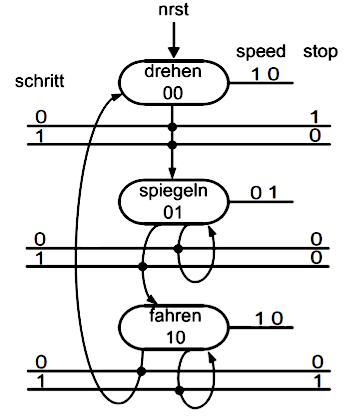
\includegraphics[width=0.15\textwidth]{pics/statediagramm}
	\end{multicols}

\subsubsection{Zustandsdiagramm}
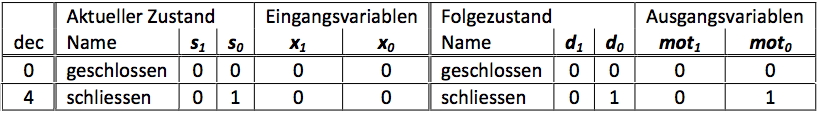
\includegraphics[width=0.6\textwidth]{pics/statetabular}
